\begin{frame}
\frametitle{Эксперимент: Rotated Drawer World, описание среды}

\begin{columns}[t]
\begin{column}{0.33\linewidth}<3->
    Пример наблюдения:
    % \begin{itemize}
    %     \item Each observation contains two entities of interest
    %     \item Each entity have its own dynamics
    %     \item Actor can directly affect or have a long-term influence over object
    % \end{itemize}
    \begin{itemize}
        \item<4-> Объектная часть
            \begin{figure}
            \begin{subfigure}{0.8\linewidth}
                \centering
                  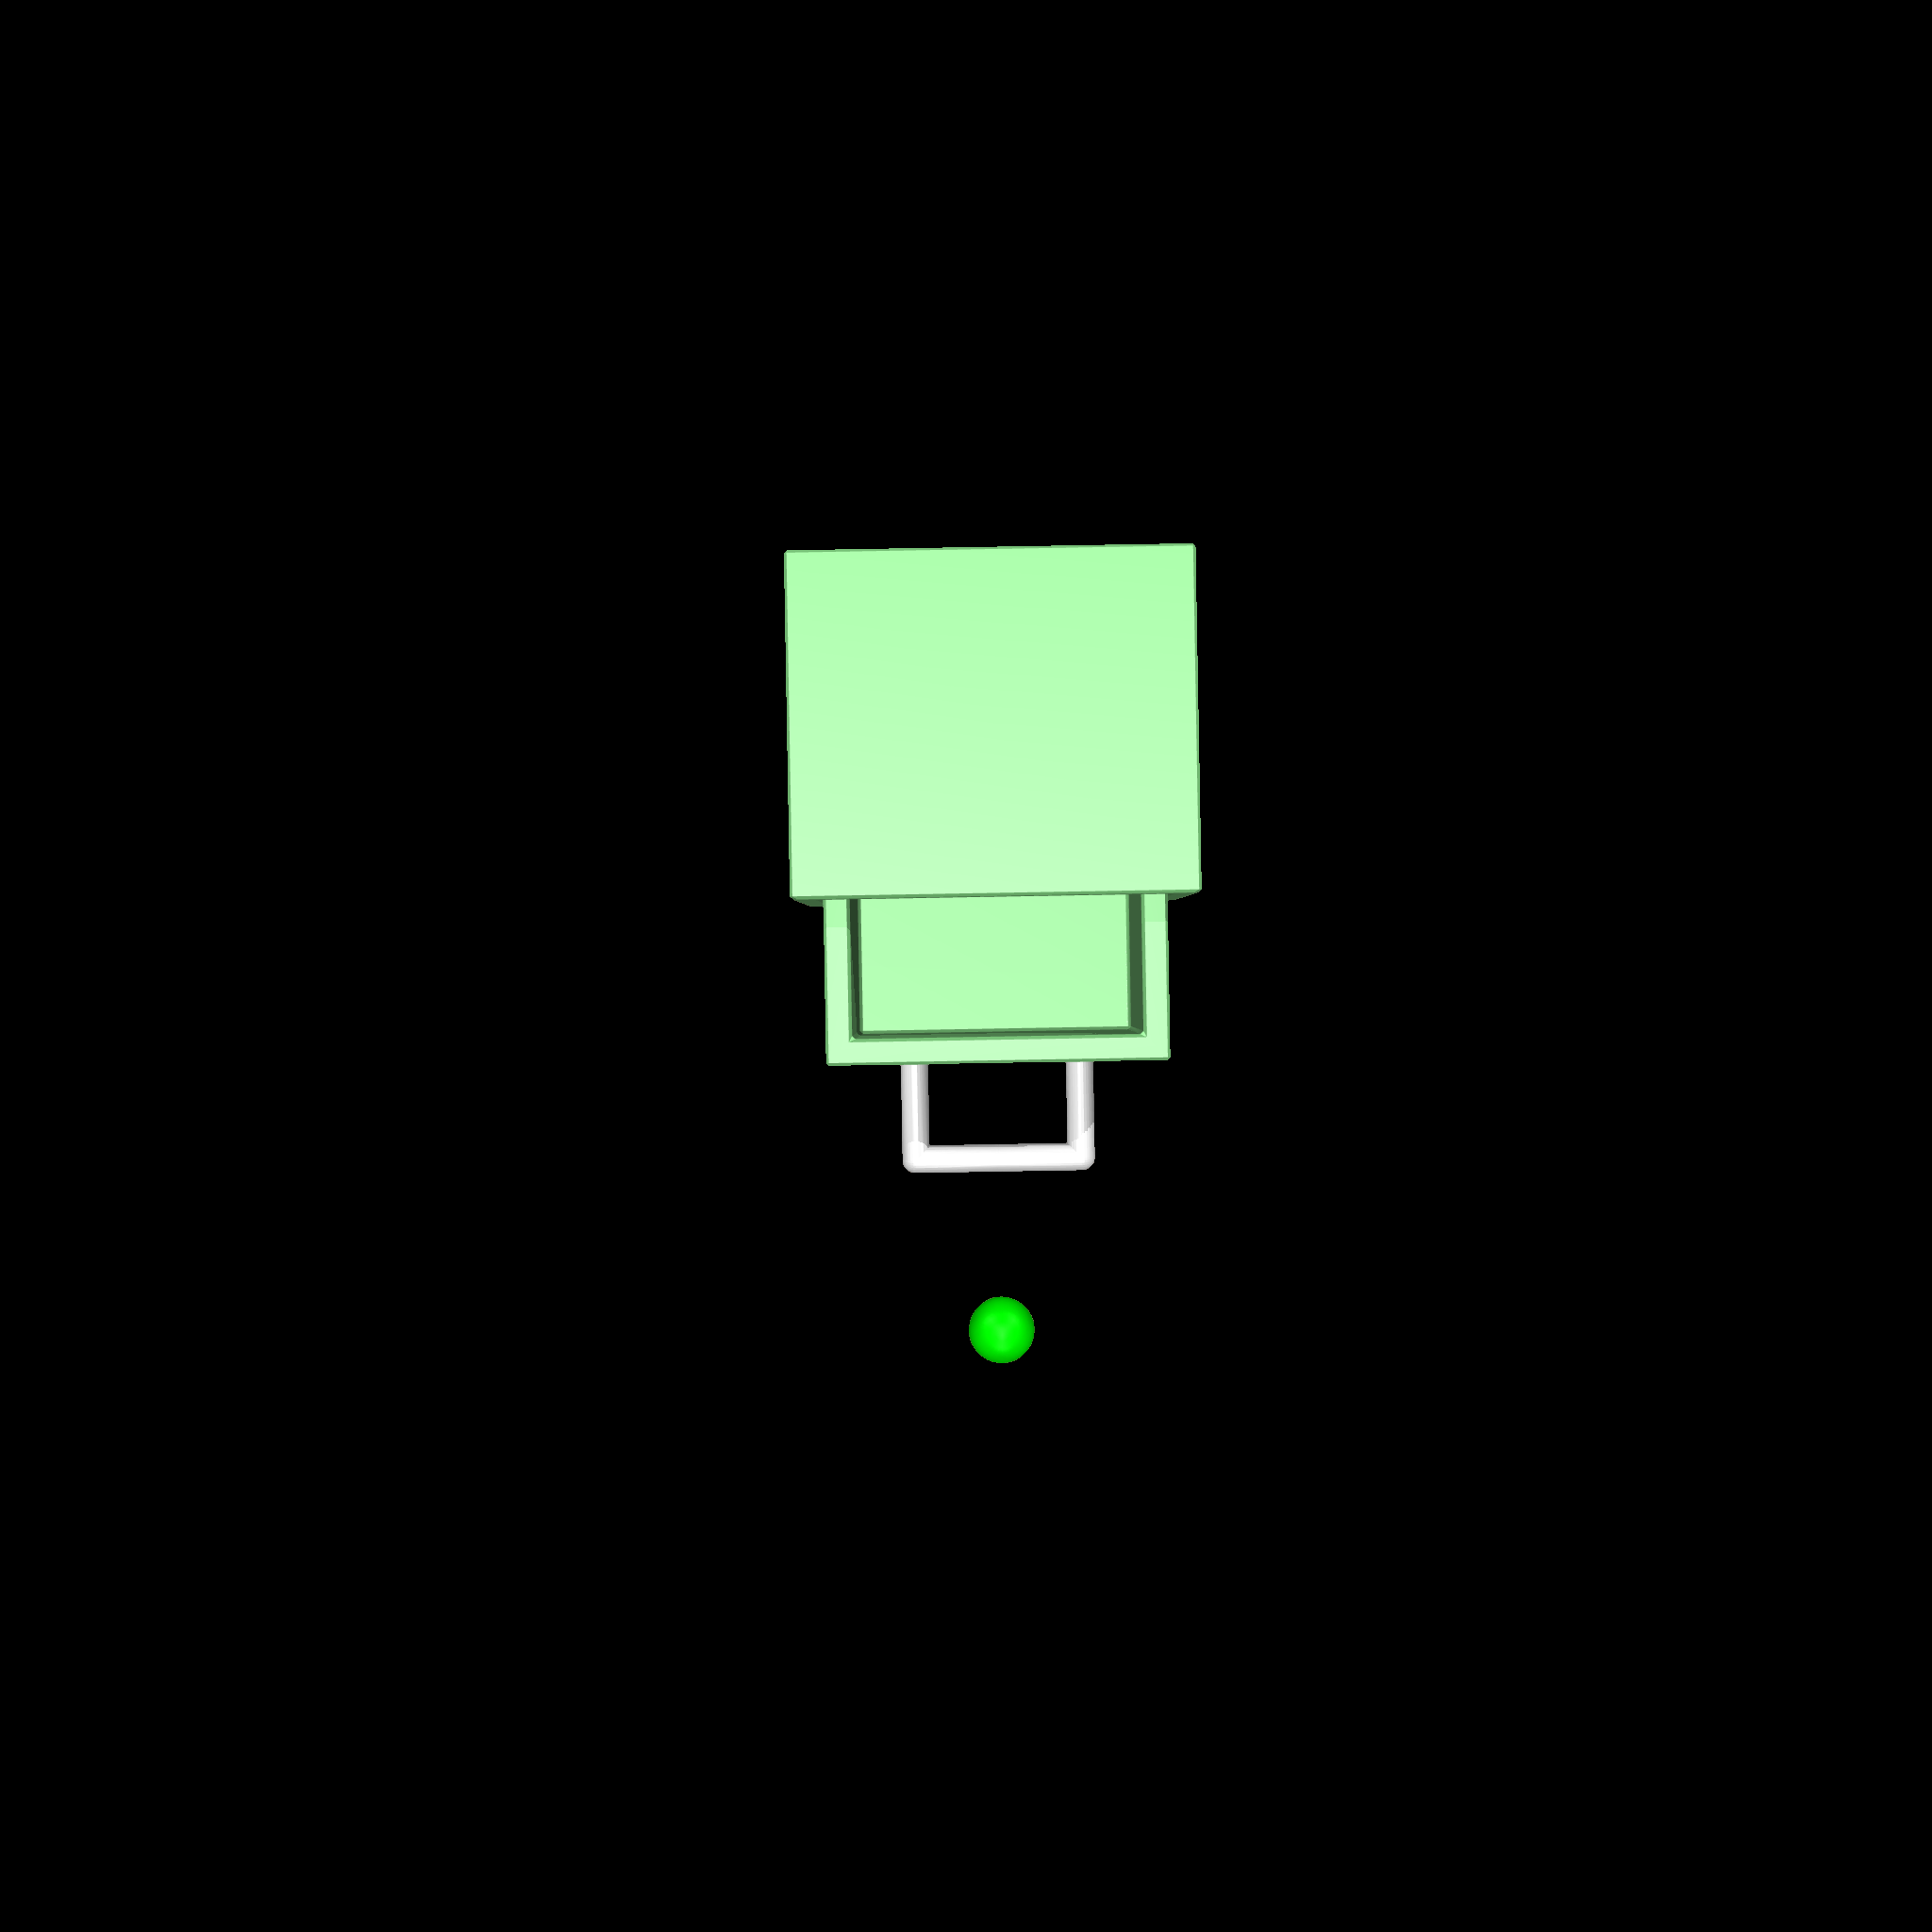
\includegraphics[width=\linewidth]{images/env/rotated_drawer/masked_obj.png}
            \end{subfigure}
            \end{figure}
        \item<5-> Субъектная часть
            \begin{figure}
            \begin{subfigure}{0.8\linewidth}
                \centering
                  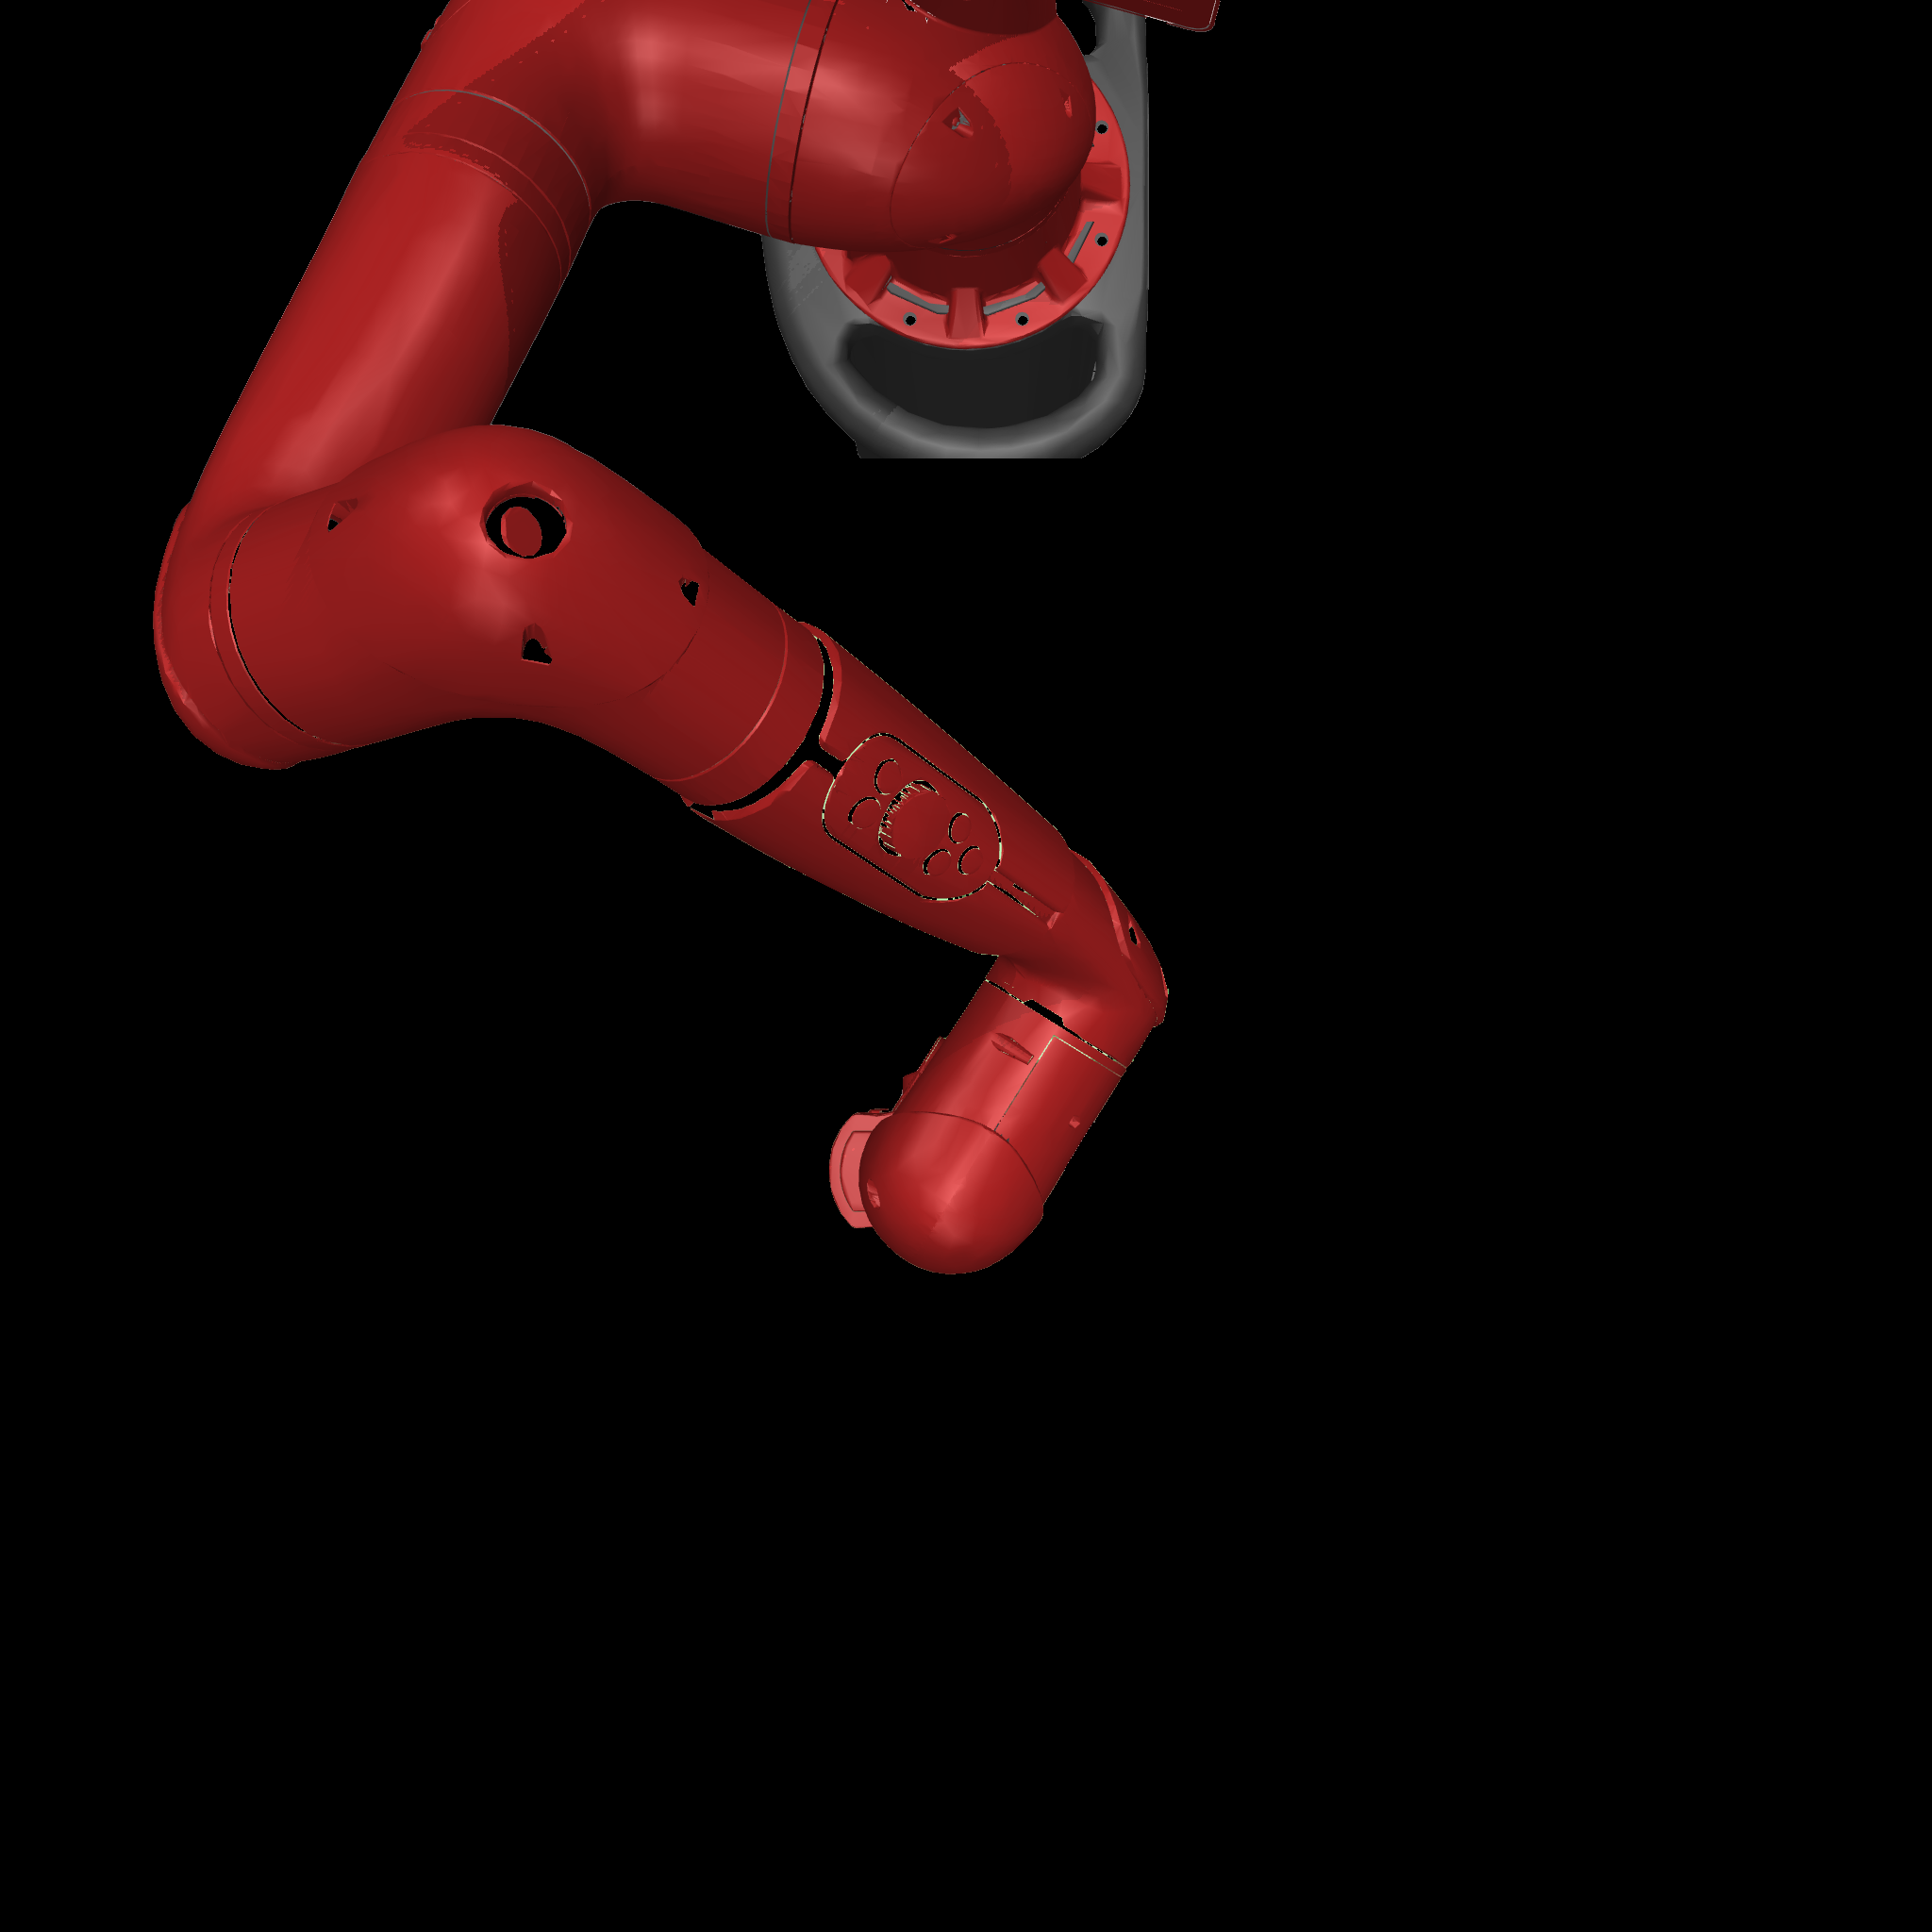
\includegraphics[width=\linewidth]{images/env/rotated_drawer/masked_robot.png}
            \end{subfigure}
            \end{figure}
    \end{itemize}
\end{column}
\hfill
\begin{column}{0.63\linewidth}<1->
    Среда для эксперимента:
    \begin{figure}
    \onslide<1->{\begin{subfigure}{.4\linewidth}
        \centering
            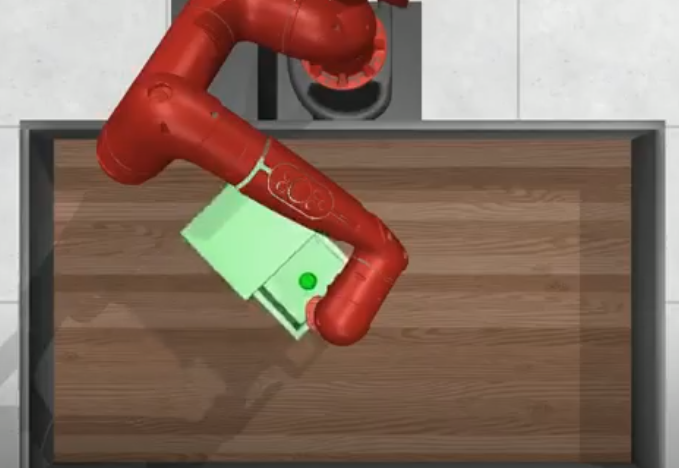
\includegraphics[width=\linewidth]{images/env/rotated_drawer/env_task2.png}
    \end{subfigure}}
    \end{figure}
    \begin{figure}
    \centering
    \onslide<2->{\begin{subfigure}{0.4\linewidth}
        \centering
            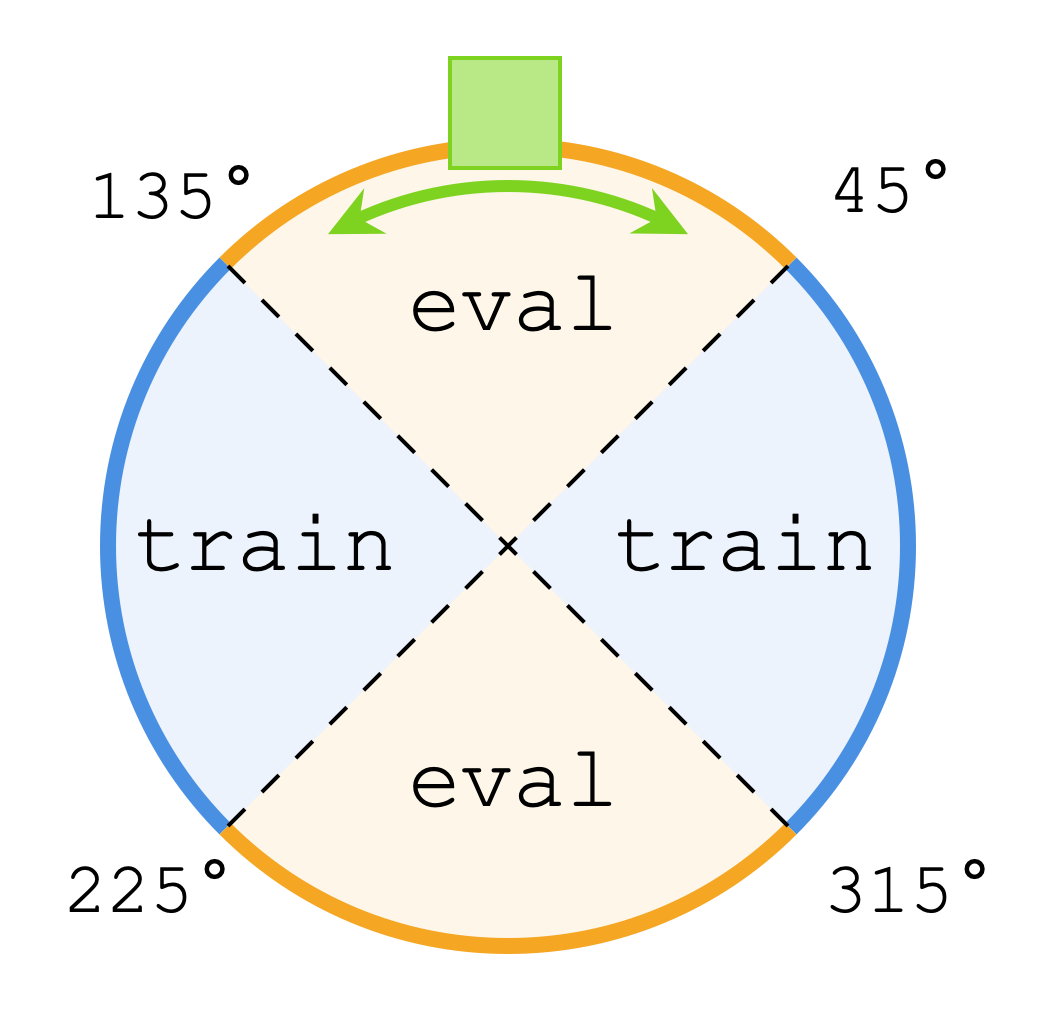
\includegraphics[width=\linewidth]{images/env/rotated_drawer/drawer_tasks.png}
    \end{subfigure}}
    \end{figure}
    \begin{figure}
        \onslide<1->{\begin{subfigure}{.4\linewidth}
            \centering
                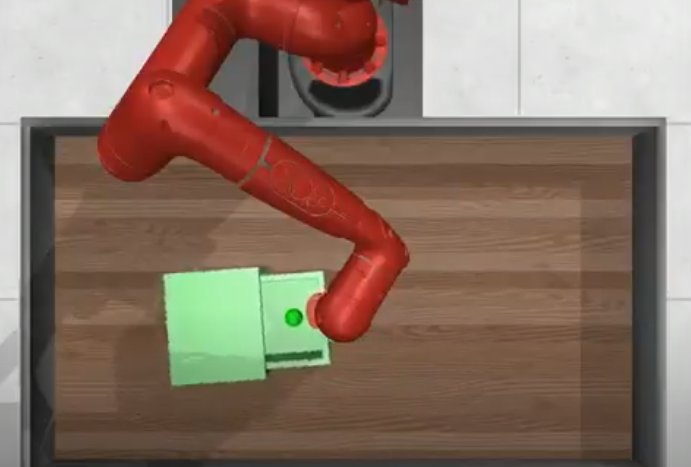
\includegraphics[width=\linewidth]{images/env/rotated_drawer/env_task1.png}
        \end{subfigure}}
        \hspace{3em}%
        \onslide<1->{\begin{subfigure}{.4\linewidth}
            \centering
                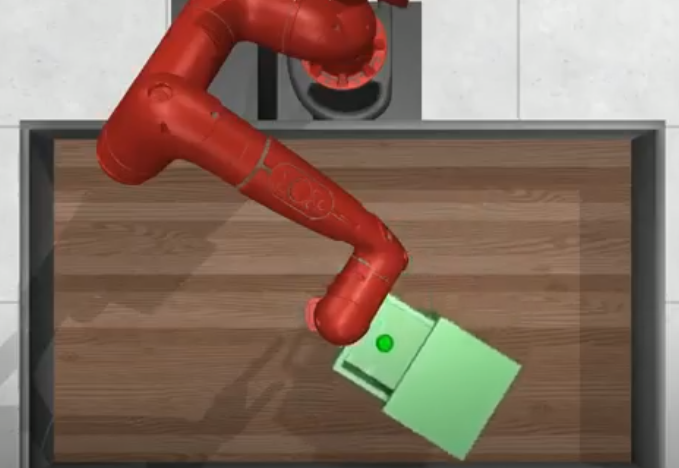
\includegraphics[width=\linewidth]{images/env/rotated_drawer/env_task3.png}
        \end{subfigure}}
    \end{figure}
    
    % Probably not needed
    % \begin{itemize}
    %     \item The task is defined by drawer position
    %     \item Ground truth segmentation masks
    %     \item Out-of-distribution test tasks
    %     \item Single topdown camera for all tasks
    % \end{itemize}
\end{column}
\end{columns}
\note[item]<1->{We built the custom parameterized task environment for evaluating the generalization capabilities of algorithm. It is a drawer, which should be opened by robotic hand.In each specific task, the drawer is fixed.}
\note[item]<2->{The set of tasks then coincides with the set of positions of the drawer, which is a circle with a given radius.}
\note[item]<3->{Each observation consists of two parts:}
\note[item]<4->{the unoccluded object image;}
\note[item]<5->{and the robot image.}
\end{frame}